%\documentclass{report}
%\usepackage[english]{babel}
\usepackage{illcmolthesis}
\usepackage{microtype}
\usepackage{amsmath,amssymb}
\usepackage{amsthm}
\usepackage[round, authoryear]{natbib}
\usepackage[all]{xy}
\usepackage{array}
\usepackage{graphicx}
\usepackage{framed}
\usepackage{enumerate}
\usepackage{qtree}
\usepackage{mdframed}
\usepackage{tikz}
\usepackage{multirow}
\usepackage{pgfplots}
\pgfplotsset{compat = newest}
\usepackage{tikz-dependency}
\usepackage{xfrac}
\usepackage{algorithmic}
\usepackage{algorithm}
\usepackage{float}
\usepackage[OT2,T1]{fontenc}
\usepackage{hyperref}
\newcommand\textcyr[1]{{\fontencoding{OT2}\fontfamily{wncyr}\selectfont #1}}
\newcommand{\myparagraph}[1]{\paragraph{#1}\mbox{}\\}
\bibliographystyle{plainnat}
\renewcommand\topfraction{0.85}
\renewcommand\bottomfraction{0.85}
\renewcommand\textfraction{0.1}
\renewcommand\floatpagefraction{0.85}

%Define theorem style for definition and metric
\newtheoremstyle{break}  % follow `plain` defaults but change HEADSPACE.
  {\topsep}   % ABOVESPACE
  {15pt}   % BELOWSPACE
  {\itshape}  % BODYFONT
  {0pt}       % INDENT (empty value is the same as 0pt)
  {\bfseries} % HEADFONT
  {.}         % HEADPUNCT
  {\newline}  % HEADSPACE. `plain` default: {5pt plus 1pt minus 1pt}
  {}          % CUSTOM-HEAD-SPEC

\theoremstyle{break}
\newtheorem{metric}{Metric}
\newtheorem{notion}{Notion}
\newtheorem{definition}{Definition}
\def\citepos#1{\citeauthor{#1}'s (\citeyear{#1})}

%Define new float environment for tables that is boxed
\floatstyle{boxed}
\newfloat{tab}{tbp}{lop}
\floatname{tab}{Table}

%\begin{document}
\chapter{Introduction}

%twee keer something?
Language and meaning play an important role in many aspects of our lives. When means of transportation and communication over larger distances became more publicly available, contact with other cultures became more prevalent and being able to understand how meanings are expressed in other languages than ones mother tongue became more important. Translation has something intriguing, as it seems to touch on something that is universal for all human beings, but is yet, even for human beings, a very nontrivial task. We would like to start this thesis with a famous quote of Warren Weaver that we believe has, besides the author of current work, inspired many to pursue a career in machine translation:

\begin{quote}
\textit{``When I look at an article in Russian, I say: `This is really written in English, but it has been coded in some strange symbols. I will now proceed to decode.''} \citep{weaver1955translation}
\end{quote}

Evidently, automatic translation is not as easily solved as Weaver thought at the time. Over 60 years later, the state-of-the-art systems are still not able to produce translations of arbitrary pieces of text with a quality comparable to that of a human translation. This was not for the lack of trying: on Google Scholar one can find over 100,000 articles that contain the phrase ``Machine Translation'', of which almost 10,000 were published in the last two years.

\section*{Compositional Translation}

One of the many different methods that have been explored over the years is called the transfer method. Contrary to more direct approaches that treat sentences as structureless sequences that can be translated into a sequence of words in another language more or less word for word, the transfer method aims to find structural representations for sentences in the source and target languages and a mapping between them. The translation process then consists of analysing the source sentence into a structure, mapping this structure to a target side structure, and generating a target sentence from this structure. A graphical representation of this process is shown in Figure \ref{fig:triangle}. The depicted pyramid shows that direct (word for word) translation can be seen as an extreme version of the transfer method, in which the distance from the sentences to the intermediate representation is zero, and thus no analysis or generation takes place. On the other end of the spectrum we can find the case in which the intermediate representation is a universal one, independent of source and target language, and the mapping is the identity mapping. Such a universal intermediate representation of language is called an `interlingua'. 


\begin{figure}[!ht]
\centering
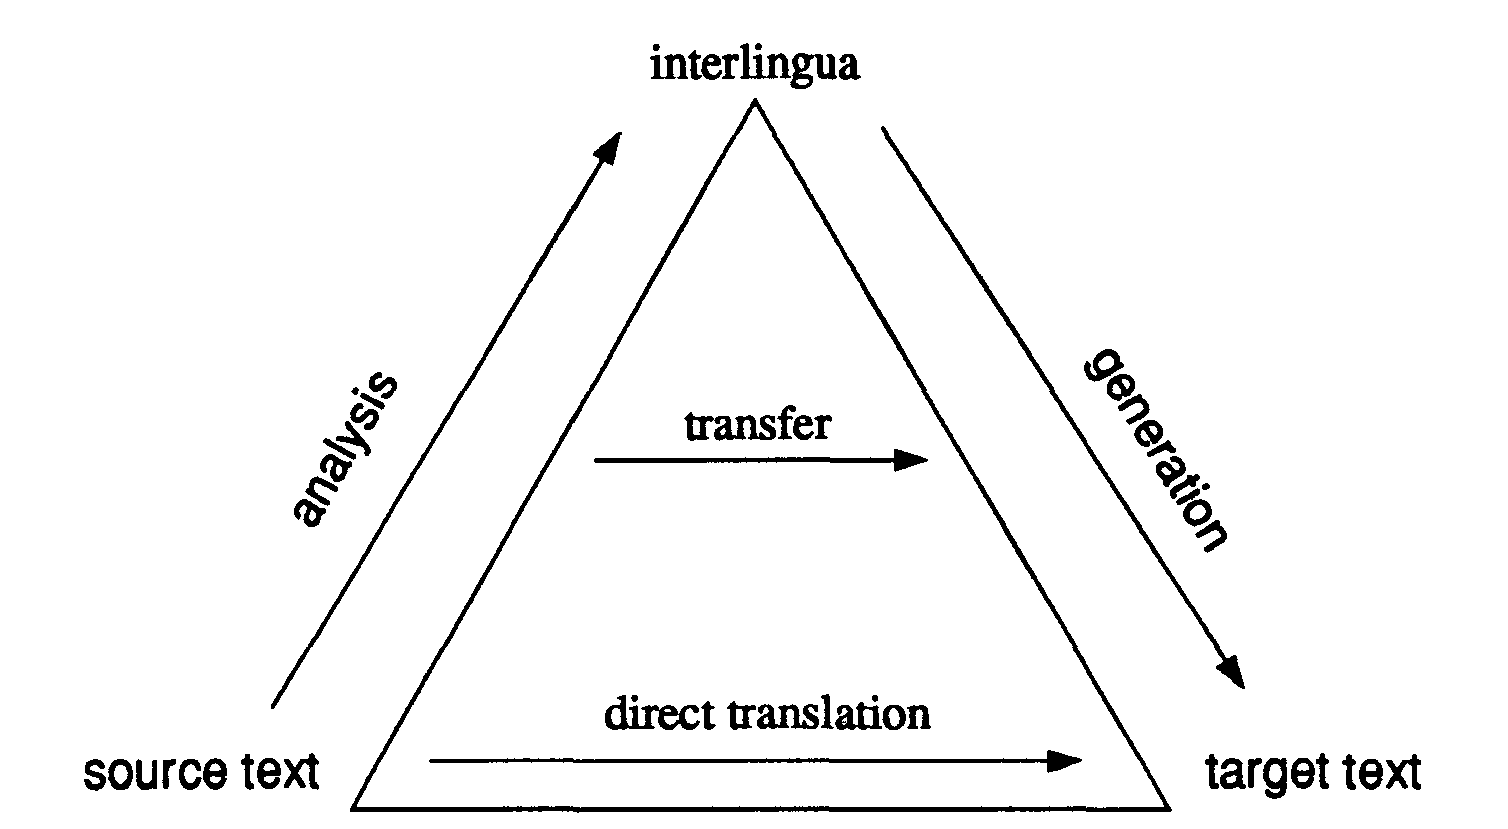
\includegraphics[scale=0.2]{Graphics/translation_triangle.png}
\caption{Vauquois pyramid}\label{fig:triangle}
\end{figure}

The pyramid also shows that transfer can be employed in many ways, varying the distance from intermediate representation to source and target language (analysis and generation, respectively). In this thesis, we consider the case in which the intermediate representations are interpreted as structural descriptions specifying how to derive the meaning of a sentence from the meaning of its parts.\footnote{Theoretically, we believe this is the only interesting case of transfer, although transferring other types of information might be useful in practice.} In other words, the underlying system generating these structures can be seen as a semantically motivated syntax of the language that specifies how the sentence was (compositionally) constructed with respect to its meaning. Hereby, it is important to notice that the system describing these structures gives a recursive notion of meaning, and a mapping between source and target structures that utilizes this fact can thus also be seen as compositional.

The type of transfer that matches compositional translation is theoretically interesting, as it addresses translation on a very fundamental level. However, although very many translation models have tried to incorporate transfer as such \citep[e.g.,][]{wu1997stochastic,chiang2005hierarchical}, and compositional methods of translation are theoretically well studied \citep[e.g.,][]{janssen1996compositionality}, it is not fully understood if translation from natural language to natural language can be treated in such a compositional fashion. In translation between other domains (logical languages, programming languages), compositional translation is almost trivially a sound approach, as the expressions of such languages are completely unambiguous and the compositional system (also called a grammar) according to which the meaning can be derived is known. Natural language has neither of these qualities, which does not only complicate the construction of a translation system, but also renders the existence of such a system uncertain.

\section*{The Adequacy of Compositional Translation}

In this thesis, we will investigate the adequacy of compositional translation as a method for translation between natural languages. As this is a very wide and well investigated question, we do not expect to solve the matter in one master thesis. Rather, we will focus on one subproblem. The research questions asked, as well as the strategies for assessing them, are founded in four core observations.

\paragraph{1.} The adequacy of compositional translation seems hard to assess by application. The soundness of the approach can only be confirmed - by a machine successfully carrying out translation - and not refuted. Although many researchers have tried, the MT world is far from presenting such a machine.

In theory, on the contrary, the soundness of compositional translation can only be refuted - by finding examples that cannot be translated as such - and not be confirmed. However, it turns out that theoretical examples of non-compositional translations (e.g., idiomatic translations), can often be dealt with elegantly in practice \citep{janssen1996compositionality}. Neither of these approaches thus seem to be promising with respect to determining whether it is possible to systematically construct structures for two languages and a mapping between them.

\paragraph{2.} The availability of huge parallel corpora with texts that are manual translations of each other, together with techniques to align these corpora on the sentence and even word level, provide a rich source of information about translation. Alignments specify, on different levels of granularity, which units are each others translation and can therefore be interpreted as constraints on the compositional structures according to which the sentence was possibly translated. These constraints, and the set of compositional structures they give rise to, can be investigated, resulting in a more suitable strategy of assessing compositional translation: empirical research.

\paragraph{3.} Previous empirical studies of translation data can be roughly divided into two categories: formal studies and linguistic studies. The former studies focus on the formal properties of the structures alignments enact. For instance, prior studies have focussed on the coverage of structures that are completely binary \citep[e.g.,][]{sogaard2009empirical1}. While such studies provide insight in the complexity of the transformation phenomena that occur during translation, their purely bilingual perspective requires arbitrary choices to prefer one compositional structure over the other.

Linguistic studies, on the other hand, study the extent to which conventional \textit{monolingual} linguistic syntax oversteps the constraints set by alignments\citep[e.g.,][]{fox2002phrasal,hwa2002evaluating}. Under this perspective, informed choices can be made as to which structures should be included in a grammar, but when alignments and monolingual syntax deviate, there is no solution available to solve this. The literature seems to lack a study that combines the strength of both approaches.

\paragraph{4.} Given their cognitive motivation and semantic nature, dependency parses seem a suitable monolingual formalism to motivate bilingual choices. Furthermore, investigating dependency parses through translation data will offer a wider perspective on its universality. However, there are no thorough studies that assess the usefulness of dependency parses for translation that take a general perspective. \cite{hwa2002evaluating} investigated whether dependency parses can be projected from English to Chinese, but did not account for unaligned words or phrasal translations. \cite{fox2002phrasal} investigated how well the phrases suggested by dependency parses cohere during translation from English to French, but constituency grammars were the main focus of her paper, and her only conclusion related to dependency parses was that they seemed more cohesive than constituency grammars.

\section*{Research Questions and Plan}

The previous observations resulted in the following research questions:\begin{enumerate}
\item Are the compositional structures suggested by dependency parses universal for language?
\item What are the reasons dependency structures deviate during translation?
\item Can dependency parses be used to construct a bilingual compositional grammar?
\end{enumerate}

We will address these questions empirically, by investigating the coherence between the dependency parse of a sentence (monolingual linguistic perspective) and \textit{all} maximally compositional translation structures that are in agreement with its alignment\footnote{As previously defined in \cite{simaan2013hats}, where they are called HATs} (bilingual formal perspective). We will investigate whether dependency relations are generally preserved during translation, and what the main causes are for parses to break down during translation. Finally, we will propose a method for combining the information from dependency parses and HATs to learn a bilingual grammar.

\section*{Contributions}
The contributions of this thesis are twofold. Firstly, we will investigate the preservation of predicate argument structures across different language pairs. As this yields an empirical view on the universality of such structures, this is interesting for the field of linguistics in general. Furthermore, the results of such research are interesting for machine translation, as they broaden the perspective on the adequacy of compositional translation as a strategy for translating from one natural language to another.

Secondly, we present an open source implementation that can be used for further research in the same direction, but also to enrich translation corpora with recursive translation structures, motivated by linguistic intuitions. The resulting structurally consistent treebank for a parallel corpus might serve as a starting point for a new MT model, and the tools provided to learn and train a grammar from this treebank could prove useful for developing one.

\section*{Thesis Outline}

This thesis is structured as follows. In Chapter 2, background information about the field of machine translation is provided. The chapter gives a general overview of the developments that led the field to its current state, and discusses techniques and models that are relevant for this thesis in more detail. In the subsequent chapter, empirical research of compositional translation is discussed. The chapter starts with setting out the main assumptions underpinning compositional translation, subsequently discusses how these can be empirically evaluated, and summarises related empirical research. The chapter ends with a background section on dependency grammars.
In Chapter 4, the research questions of this thesis will be revisited, and more extensively discussed. Furthermore, Chapter 4 presents the basic algorithms and strategies that are used to answer these questions. The actual experiments, as well as their results, will be discussed in Chapter 5. In Chapter 6, we will look back at the thesis, discuss its results, and propose a method for overcoming the problems that were encountered in previous chapters. Examples from the data and documentation of the implementation can be found in Appendix A and B, respectively.



%\bibliography{thesisDH}
%\end{document}